%%%%%%%%%%%%%%%%%%%%%%%%%%%%%%%%%%%%%%%%%
% a0poster Portrait Poster
% LaTeX Template
% Version 1.0 (22/06/13)
%
% The a0poster class was created by:
% Gerlinde Kettl and Matthias Weiser (tex@kettl.de)
% 
% This template has been downloaded from:
% http://www.LaTeXTemplates.com
%
% License:
% CC BY-NC-SA 3.0 (http://creativecommons.org/licenses/by-nc-sa/3.0/)
%
%%%%%%%%%%%%%%%%%%%%%%%%%%%%%%%%%%%%%%%%%

%----------------------------------------------------------------------------------------
%	PACKAGES AND OTHER DOCUMENT CONFIGURATIONS
%----------------------------------------------------------------------------------------

\documentclass[a0,portrait]{a0poster}

\usepackage{multicol} % This is so we can have multiple columns of text side-by-side
\columnsep=100pt % This is the amount of white space between the columns in the poster
\columnseprule=3pt % This is the thickness of the black line between the columns in the poster

\usepackage[svgnames]{xcolor} % Specify colors by their 'svgnames', for a full list of all colors available see here: http://www.latextemplates.com/svgnames-colors

\usepackage{times} % Use the times font
%\usepackage{palatino} % Uncomment to use the Palatino font

\usepackage{graphicx} % Required for including images
\graphicspath{{figures/}, {../images/}} % Location of the graphics files
\usepackage{booktabs} % Top and bottom rules for table
\usepackage[font=small,labelfont=bf]{caption} % Required for specifying captions to tables and figures
\usepackage{amsfonts, amsmath, amsthm, amssymb} % For math fonts, symbols and environments
\usepackage{wrapfig} % Allows wrapping text around tables and figures


\usepackage[T1]{fontenc}
\usepackage[utf8]{inputenc}
\usepackage{lmodern} 
\usepackage[portuguese]{babel}%para podermos usar o bom e velho portugues

\usepackage{graphicx}				%para imagens
\usepackage{epstopdf} 				%resolve problemas eps-pdf
\usepackage{pict2e}				%%writting to images

\usepackage[import]{xy} % para escrever em imagens
\xyoption{import}

\usepackage{placeins} %controla o lugar dos floats com \FloatBarrier

\begin{document}

%----------------------------------------------------------------------------------------
%	POSTER HEADER 
%----------------------------------------------------------------------------------------

% The header is divided into two boxes:
% The first is 75% wide and houses the title, subtitle, names, university/organization and contact information
% The second is 25% wide and houses a logo for your university/organization or a photo of you
% The widths of these boxes can be easily edited to accommodate your content as you see fit

\begin{minipage}[b]{0.75\linewidth}
\veryHuge \color{NavyBlue} \textbf{Introdução à Simulação Híbrida\\ de
Escoamentos de 
Partículas em Fluidos} \color{Black}\\ % Title
\Huge\textit{Dinâmica Molecular}\\[2cm] % Subtitle
\huge \textbf{Juarez Aires Sampaio Filho}\\[0.5cm] % Author(s)
\huge Universidade de Brasília - Departamento de Matemática\\[0.4cm] % University/organization
%\Large \texttt{john@LaTeXTemplates.com} --- 1 (000) 111 1111\\
\end{minipage}
%
\begin{minipage}[b]{0.25\linewidth}

\includegraphics[width = 10cm]{../images/as_vert_PB.jpg}\\
\end{minipage}

\vspace{1cm} % A bit of extra whitespace between the header and poster content

%----------------------------------------------------------------------------------------

\begin{multicols}{2} % This is how many columns your poster will be broken into, a portrait poster is generally split into 2 columns

%----------------------------------------------------------------------------------------
%	ABSTRACT
%----------------------------------------------------------------------------------------

%\color{Navy} % Navy color for the abstract

%\begin{abstract}

%COLOQUE AQUI O RESUMO
%\end{abstract}

%----------------------------------------------------------------------------------------
%	INTRODUCTION
%----------------------------------------------------------------------------------------

\color{SaddleBrown} % SaddleBrown color for the introduction

\section*{Introduction}
\paragraph{} O comportamento da mistura que se forma quando fazemos passar
um fluído por um material granular ainda não foi completamente 
entendido. Uma das ferramentas atualmente utilizadas para o estudo de tal
fenômeno é a simulação computacional. Para isso precisamos ser capazes
de descrever as interações das partículas granulares entre si e do fluído
com as partículas.
\paragraph{}A interação entre as partículas do material granular pode
ser simulada pelo uso da dinâmica molecular. Essa técnica consiste em 
fornecer um modelo para as forças de interação trocadas entre as partículas
em colisão. A partir dessas forças a equação de movimento pode ser integrada 
numericamente e obtém-se a trajetória de cada partícula individualmente.
\paragraph{}A simulação do fluído é baseada nas equações
de Navier-Stokes. Para resolvermos numericamente as equações utilizamos
diferenças finitas, técnica por meio da qual transforma-se a solução da
equação diferencial na solução de um conjunto de sistemas lineares.

\color{DarkSlateGray} % DarkSlateGray color for the rest of the content


%----------------------------------------------------------------------------------------
%	MATERIALS AND METHODS
%----------------------------------------------------------------------------------------

\section*{Metodologia}

\paragraph{}O trabalho realizado focou a primeira etapa dos processos
envolvidos na simulação computacional do escoamento de partículas em fluídos,
isto é, a simulação da interação entre partículas por meio da dinâmica
molecular e as dificuldades de uma implementação eficiente. Descrevemos a seguir
as ideias chaves utilizadas.
%------------------------------------------------
\subsection*{Dinâmica Molecular}
\paragraph{} Essa técnica fornece um modelo para as forças envolvidas nos
instantes de colisão. Para isso, o material granular é visto como um conjunto
de partículas circulares capazes de sofrerem deformação. Essa deformação é
simulada deixando que as partículas sofram interpenetrações elásticas $ \xi $,
isto é,
durante uma colisão permitimos que as partículas possuam áreas de superposição,
mas essas áreas de superposição produzem forças no sentido de afastá-las. O
comportamento dessa força é representado pela lei de Hooke com constante 
elástica $k_{r}$ e constante de amortecimento $k_{v}$.

\vspace{-2cm}
\begin{minipage}{0.25\textwidth}
\paragraph{}As principais grandezas físicas utilizadas
  são mostradas na figura ao lado.
  Sejam $\vec{x_1}$ e $\vec{x_2}$ as posições,
  $R_1$ e $R_2$ os raios,  $\vec{v_1}$ e $\vec{v_2}$
  as velocidade  das
  partículas 1 e 2 respectivamente e $\vec{n}$ e
  $\vec{t}$ as direções normais e tangentes. Temos:
  \begin{equation}
  \left\{
    \begin{array}{l}
      \mbox{(overlap)}
              \xi
              = max(0, R_1 + R_2 - |\vec{x_2} - \vec{x_1} |)
		    \\%	
	      \mbox{(direção normal)}
			\vec{N} = \frac{\vec{x_2} -
			\vec{x_1} }{|\vec{x_2} - \vec{x_1} |}
	      \\ %	
	      \mbox{ (v de aproximação)}\vec{V} = \vec{v_1} - \vec{v_2}
	      \\%	
	      \mbox{ (v normal)}  V_n = \dot{\xi} = \vec{V} \cdot \vec{N} 
	      \\%	
	      \mbox{ (v tang.)}  \vec{V}_t = \vec{V} - \dot{\xi}\vec{N} 
	      \\%
	       \vec{F}_n = f_n \vec{N}, \\
	    	f_n = -(k_v \xi^\alpha \dot{\xi} + k_r \xi^\beta)

	\end{array}\right.
	\label{eq:DM-1}
  \end{equation}
 
\end{minipage}
\begin{minipage}{0.25\textwidth}
\begin{center}\vspace{1cm}
\centering
       \setlength{\unitlength}{0.08\textwidth}
       \begin{picture}(10,9)
	\put(0,0){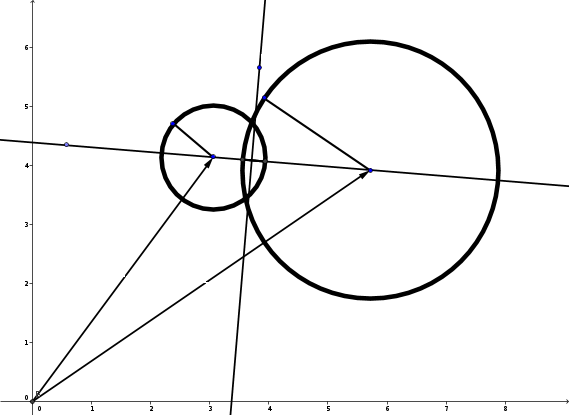
\includegraphics[width=0.8\textwidth]{../images/fig_1-1.png}}
                \put(2.5,3.5){$ \vec{x_1}$}
                \put(3.0, 2.5){$\vec{x_2}$}
                \put(5.2, 5.0){$\vec{R_2}$}
               \put(3.2, 4.8){$\vec{R_1}$}
                \put(4.3, 4.4){$\xi$}

          \end{picture}
	\label{fig:MD}
	\captionof{figure}{\color{Green} modelo para simulação de forças de
colisão}
\end{center}\vspace{1cm}

\end{minipage}

\subsection*{Tabela de Dispersão}
\vspace{-2cm}
\begin{minipage}{0.25\textwidth}
\paragraph{}Um dos problemas computacionais envolvidos na simulação é a
detecção de colisões de forma eficiente. Detectar colisões significa medir a
distância entre todas as partículas e determinar qual destas é menor que a soma
dos raios das partículas envolvidas, o problema é que, a princípio, todas as
partículas são candidatas a colidirem com todas as outras e teríamos de
verificar todos os pares possíveis. Gostaríamos de reduzir o número de pares
candidatos a colisão ao procurarmos apenas naquelas partículas que estão
próximas umas das outras. Um modo de fazer isso é pelo uso de uma tabela de
dispersão. Por meio dessa técnica segmentamos o plano em quadrados e, para
uma dada partícula, procuramos apenas por colisões nos quadrados vizinhos. 
Para que isso seja possível, o lado do quadrado deve ser igual ao maior
diâmetro encontrado nas partículas sendo simuladas.
\end{minipage}
\begin{minipage}{0.25\textwidth}
\begin{center}\vspace{3cm}
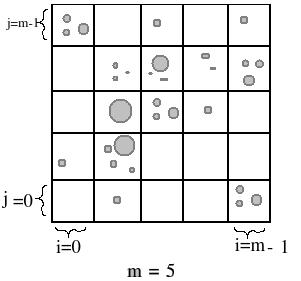
\includegraphics[width=0.8\linewidth]{../images/hash.jpeg}
\captionof{figure}{\color{Green} segmentação do plano}
\end{center}\vspace{1cm}
\end{minipage}

\subsection*{Integração Temporal}
\vspace{-1cm}
\begin{minipage}{0.25\textwidth}
\paragraph{}Depois de calculadas as colisões e as forças envolvidas, integramos
a 2ª lei de Newton para obter o movimento. No trabalho realizado
utilizamos métodos de primeira e de segunda ordem. As equações utilizadas são
mostradas ao lado. Ao utilizar o método de 2ª ordem conseguimos obter bons
resultados utilizando incrementos de tempo relativamente altos quando
comparados com os incrementes necessários para fazer o método de 1ª ordem
funcionar adequadamente.
\end{minipage}
\begin{minipage}{0.25\textwidth}
\begin{center}\vspace{3cm}
	\begin{displaymath}
	    \begin{array}{l}
		    \mbox{1ª ordem}	
			    \left\{
				      \begin{array}{l}
				      s^{(n+1)} = s^{(n)} + v^{(n)} \Delta t  
					\\
				      v^{(n+1)} = v^{(n)} + a^{(n)} \Delta t  
					  \\
				      \end{array}
			  \right. 
		  \\
		      \mbox{2ª ordem}
			    \left\{
				      \begin{array}{l}
				      s^{(n+1)} = s^{(n-1)} + 2 v^{(n)} \Delta t
 					\\
				      v^{(n+1)} = v^{(n-1)} + 2 a^{(n)} \Delta t
 				      \\
				      \end{array}
			      \right.
	    \end{array}
		\end{displaymath}		
\end{center}\vspace{1cm}
\end{minipage}

%----------------------------------------------------------------------------------------
%	RESULTS 
%----------------------------------------------------------------------------------------
\vspace{-2cm}
\section*{Resultados}
\paragraph{}Os resultados simulados são mostrados a seguir.
Na figura \ref{fig:sequenciaBloco} deixamos um bloco compacto de 500 partículas
atingir o solo a partir do repouso em uma pequena altura. A sequência mostra o
bloco instantes antes e depois do choque com a superfície e a degeneração do
bloco.

\FloatBarrier
\vspace{-2cm}
\begin{center}\vspace{3cm}
\begin{tabular}{ll}
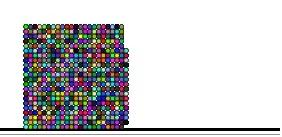
\includegraphics[width=0.3\linewidth]{../images/seq01.jpg} &
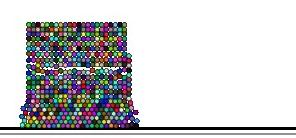
\includegraphics[width=0.3\linewidth]{../images/seq02.jpg} \\
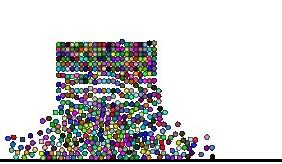
\includegraphics[width=0.3\linewidth]{../images/seq03.jpg} &
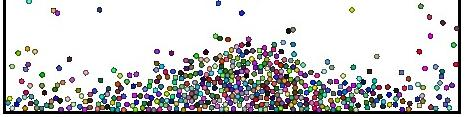
\includegraphics[width=0.4\linewidth]{../images/seq04.jpg} \\
\end{tabular}
\captionof{figure}{\color{Green} bloco compacto atinge o solo}
\label{fig:sequenciaBloco}
\end{center}
\FloatBarrier

\paragraph{}Na figura \ref{fig:sequenciaBloco2} colidimos um bloco denso móvel
menor com um bloco denso maior inicialmente em repouso. A sequência mostra
instantes imediatamente antes e depois da colisão e a degeneração dos blocos.

\FloatBarrier
\begin{center}\vspace{3cm}
\begin{tabular}{ll}
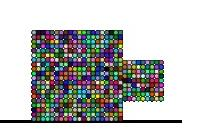
\includegraphics[width=0.3\linewidth]{../images/seq2-1.jpg} &
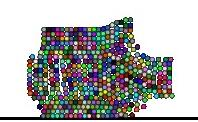
\includegraphics[width=0.3\linewidth]{../images/seq2-2.jpg} \\
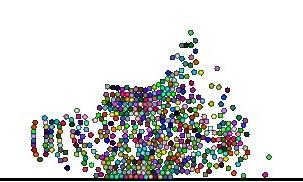
\includegraphics[width=0.3\linewidth]{../images/seq2-3.jpg} &
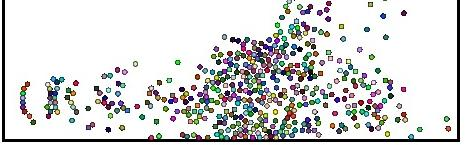
\includegraphics[width=0.4\linewidth]{../images/seq2-4.jpg} \\
\end{tabular}
\captionof{figure}{\color{Green} bloco compacto atinge o solo}
\label{fig:sequenciaBloco2}
\end{center}\vspace{1cm}
\FloatBarrier



\paragraph{}Na figura \ref{fig:grafico} vemos um gráfico comparando o algoritmo
desenvolvido de procura por colisões com hash e o algoritmo trivial de cálculo
de todos os pares possíveis. Os dados experimentais são marcados como pontos e
as linhas contínuas são regressões feitas sobres os dados. O gráfico e a
regressão obtida nos mostram que nosso algoritmo baseado em hash é linear,
enquanto o algoritmo trivial é quadrático. Outra
vantagem de nosso algoritmo é que ele é insensível ao número de partículas nas
paredes. Ou seja, o custo computacional é função apenas das partículas móveis,
diferentemente do algoritmo trivial, onde todas as partículas entram na conta
do custo.
\FloatBarrier
    \begin{center}\vspace{3cm}
	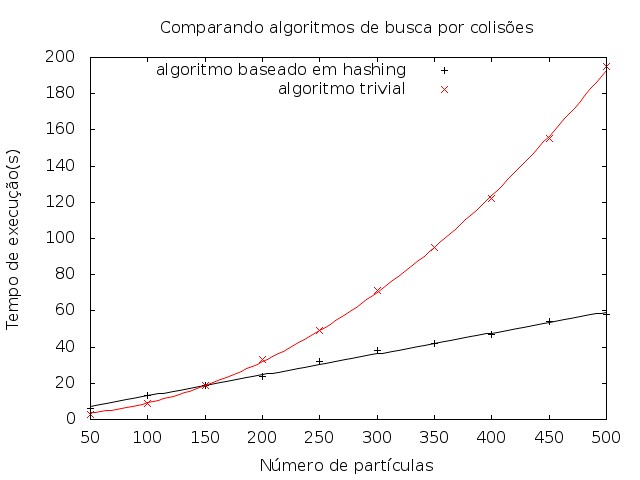
\includegraphics[scale = 1.0]{../images/comparandoAlgoritmos.jpg}
	\captionof{figure}{\color{Green} comparando o algoritmo desenvolvido}
	\label{fig:grafico}
    \end{center}\vspace{1cm}
\FloatBarrier

%----------------------------------------------------------------------------------------
%	CONCLUSIONS
%----------------------------------------------------------------------------------------

\color{SaddleBrown} % SaddleBrown color for the conclusions to make them stand out

\section*{Conclusões}

\begin{itemize}
\item O uso de Dinâmica Molecular provê um método simples para simulação de
material granular.
\item A calibração das constantes envolvidas é etapa importante no
desenvolvimento de um simulador.
\item A utilização de uma tabela de dispersão reduz o custo computacional para
determinação de colisões.
\item O custo computacional para se atingir bons resultados pode ser reduzido
ao utilizarmos algoritmos de integração temporal de ordem mais alta. Dessa
forma podemos utilizar incrementos de tempo maior em troca de precisarmos de
mais memória para guardar instantes de tempo anteriores.
\end{itemize}

\color{DarkSlateGray} % Set the color back to DarkSlateGray for the rest of the content

%----------------------------------------------------------------------------------------
%	FORTHCOMING RESEARCH
%----------------------------------------------------------------------------------------

\section*{Pesquisa Futura}
%Forthcoming Research
\paragraph{} Tendo desenvolvido o simulador para trabalhar com a dinâmica de
materiais granulares, a continuação do trabalho é resolver numericamente as
equações que regem os fluídos para então simular a interação fluído-partícula.
Dentre as ferramentas a serem utilizadas para o equacionamento do fluído estão:
diferenças finitas, para lidar com equações diferenciais, métodos de solução
iterativa de sistemas lineares e o algoritmo de Chorin para solução de
Navier-Stokes. 



\end{multicols}
\end{document}